\documentclass[a4paper,11pt,dvipdfmx]{ujarticle}

\usepackage{graphicx}
\usepackage{url}
\input{layout}

\title{インターネットの利用状況}

\author{G584502025 佐藤真優}

\begin{document}

\maketitle

\section{情報通信機器の保有状況}

総務省が毎年実施している通信利用動向調査\cite{soumu}によると,
図\ref{fig:保有率}に示すように,
情報通信機器の世帯保有率については,
携帯電話やスマートフォンなどのモバイル端末では,9割を越えている.
その中でも,スマートフォンの普及が進んでおり,8割以上の世帯で保有している.

\begin{figure}[htbp]
    \centering
    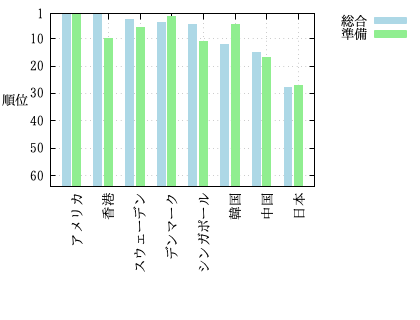
\includegraphics[width=0.7\linewidth]{fig51.png}

    \caption{デジタル競争力ランキング(64カ国中)}\label{fig:保有率}
\end{figure}

\section{端末の利用状況}

普段,私的な用途のために利用している端末で最も多いのは,
表\ref{tbl:利用状況}に示すように,
スマートフォン(89.4\%)で全体の9割近くが利用していた.
続いて,テレビ(50.8\%),ノートPC(48.5\%),タブレット(26.5\%)
の順で多く,テレビを除くと,持ち運びできる端末の利用が多い\cite{corona}.

\begin{table}[htbp]
    \centering
    \caption{インターネット端末の利用状況}
    \label{tbl:利用状況}

    \begin{tabular}{|l|r|}\hline
        端末の種類 & 利用状況(\%) \\
        \hline
        スマートフォン & 89.4 \\
        \hline
        従来型の携帯電話 & 7.0 \\
        \hline
        タブレット & 26.5 \\
        \hline
        ノートPC & 48.5 \\
        \hline
        デスクトップPC & 20.9 \\
        \hline
        ゲーム機 & 11.4 \\
        \hline 
        テレビ & 50.8 \\
        \hline
    \end{tabular}
\end{table}

\section{インターネットを利用したサービスの利用状況}

インターネットを利用したサービスについて,普段の利用状況について尋ねた結果\cite{corona}の上位は次のようになっている.
\begin{itemize}
    \item 「インターネットショッピング」(73.4\%)
    \item 「支払い・決済(クレジットカード等)」(66.9\%)
    \item 「地図・ナビゲーション」(61.4\%)
    \item 「情報検索・ニュース」(57.9\%)
    \item 「動画配信」(55.6\%)
\end{itemize}
インターネットの活用は日常生活に浸透しているといえる.
その中でも,特にインターネットショッピング,支払い・決済,動画配信等の生活や
エンターテインメント関係の利用が中心となっていることがわかる.

\bibliographystyle{junsrt}
\bibliography{exercise.bib}

\end{document}